\documentclass[twoside]{book}

% Packages required by doxygen
\usepackage{calc}
\usepackage{doxygen}
\usepackage{graphicx}
\usepackage[utf8]{inputenc}
\usepackage{makeidx}
\usepackage{multicol}
\usepackage{multirow}
\usepackage{textcomp}
\usepackage[table]{xcolor}

% NLS support packages
\usepackage[brazil]{babel}
% Font selection
\usepackage[T1]{fontenc}
\usepackage{mathptmx}
\usepackage[scaled=.90]{helvet}
\usepackage{courier}
\usepackage{amssymb}
\usepackage{sectsty}
\renewcommand{\familydefault}{\sfdefault}
\allsectionsfont{%
  \fontseries{bc}\selectfont%
  \color{darkgray}%
}
\renewcommand{\DoxyLabelFont}{%
  \fontseries{bc}\selectfont%
  \color{darkgray}%
}

% Page & text layout
\usepackage{geometry}
\geometry{%
  a4paper,%
  top=2.5cm,%
  bottom=2.5cm,%
  left=2.5cm,%
  right=2.5cm%
}
\tolerance=750
\hfuzz=15pt
\hbadness=750
\setlength{\emergencystretch}{15pt}
\setlength{\parindent}{0cm}
\setlength{\parskip}{0.2cm}
\makeatletter
\renewcommand{\paragraph}{%
  \@startsection{paragraph}{4}{0ex}{-1.0ex}{1.0ex}{%
    \normalfont\normalsize\bfseries\SS@parafont%
  }%
}
\renewcommand{\subparagraph}{%
  \@startsection{subparagraph}{5}{0ex}{-1.0ex}{1.0ex}{%
    \normalfont\normalsize\bfseries\SS@subparafont%
  }%
}
\makeatother

% Headers & footers
\usepackage{fancyhdr}
\pagestyle{fancyplain}
\fancyhead[LE]{\fancyplain{}{\bfseries\thepage}}
\fancyhead[CE]{\fancyplain{}{}}
\fancyhead[RE]{\fancyplain{}{\bfseries\leftmark}}
\fancyhead[LO]{\fancyplain{}{\bfseries\rightmark}}
\fancyhead[CO]{\fancyplain{}{}}
\fancyhead[RO]{\fancyplain{}{\bfseries\thepage}}
\fancyfoot[LE]{\fancyplain{}{}}
\fancyfoot[CE]{\fancyplain{}{}}
\fancyfoot[RE]{\fancyplain{}{\bfseries\scriptsize Gerado em Quinta, 3 de Março de 2016 19\-:04\-:39 para Parameters por Doxygen }}
\fancyfoot[LO]{\fancyplain{}{\bfseries\scriptsize Gerado em Quinta, 3 de Março de 2016 19\-:04\-:39 para Parameters por Doxygen }}
\fancyfoot[CO]{\fancyplain{}{}}
\fancyfoot[RO]{\fancyplain{}{}}
\renewcommand{\footrulewidth}{0.4pt}
\renewcommand{\chaptermark}[1]{%
  \markboth{#1}{}%
}
\renewcommand{\sectionmark}[1]{%
  \markright{\thesection\ #1}%
}

% Indices & bibliography
\usepackage{natbib}
\usepackage[titles]{tocloft}
\setcounter{tocdepth}{3}
\setcounter{secnumdepth}{5}
\makeindex

% Hyperlinks (required, but should be loaded last)
\usepackage{ifpdf}
\ifpdf
  \usepackage[pdftex,pagebackref=true]{hyperref}
\else
  \usepackage[ps2pdf,pagebackref=true]{hyperref}
\fi
\hypersetup{%
  colorlinks=true,%
  linkcolor=blue,%
  citecolor=blue,%
  unicode%
}

% Custom commands
\newcommand{\clearemptydoublepage}{%
  \newpage{\pagestyle{empty}\cleardoublepage}%
}


%===== C O N T E N T S =====

\begin{document}

% Titlepage & ToC
\hypersetup{pageanchor=false}
\pagenumbering{roman}
\begin{titlepage}
\vspace*{7cm}
\begin{center}%
{\Large Parameters \\[1ex]\large 1.\-0 }\\
\vspace*{1cm}
{\large Gerado por Doxygen 1.8.6}\\
\vspace*{0.5cm}
{\small Quinta, 3 de Março de 2016 19:04:39}\\
\end{center}
\end{titlepage}
\clearemptydoublepage
\tableofcontents
\clearemptydoublepage
\pagenumbering{arabic}
\hypersetup{pageanchor=true}

%--- Begin generated contents ---
\chapter{Este projeto permite armazenar parâmetros em arquivos.}
\label{index}\hypertarget{index}{}\begin{DoxyAuthor}{Autor}
Hansenclever Bassani
\end{DoxyAuthor}
As três classes principais são\-:

\hyperlink{class_parameters}{Parameters}\-: define um conjunto de parâmetros

\hyperlink{class_parameter}{Parameter}\-: define um parâmetro

\hyperlink{class_c_f_g_file}{C\-F\-G\-File}\-: define um arquivo onde os parâmetros serão armazenados.

Exemplo de utilização\-: 
\begin{DoxyCode}
\textcolor{comment}{//Primeiramente é necessário definir uma classe derivada de Parameters que irá conter os parâmetros:}
 
\textcolor{keyword}{class }MyParameters: \textcolor{keyword}{public} \hyperlink{class_parameters}{Parameters} \{

\textcolor{keyword}{public}:
     \textcolor{comment}{//Esta classe contém três parâmetros:}
     \hyperlink{class_parameter}{Parameter<double>} p1; \textcolor{comment}{//parametro double}
     \hyperlink{class_parameter}{Parameter<float>} p2;  \textcolor{comment}{//parametro float}
     \hyperlink{class_parameter}{Parameter<int>} p3;    \textcolor{comment}{//parametro inteiro}

     \textcolor{comment}{//Em seguida definimos um construtor da seguinte maneira:}
     MyParameters() \{
         \textcolor{comment}{//Um nome para este cojunto de parâmetros.}
         section = \textcolor{stringliteral}{"Meus Parametros"};

         \textcolor{comment}{//Uma descrição mais detalhada para este conjunto de parâmetros.}
         comments = \textcolor{stringliteral}{"Parametros do meu sistema p1 p2 e p3"};

         \textcolor{comment}{//Indica quais parâmetros serão salvos em arquivo e um comentário }
         \textcolor{comment}{//explicativo para cada parâmetro que será incluído no arquivo.}
         addParameterD(p1, \textcolor{stringliteral}{"Este parametro controla 1"});
         addParameterD(p2, \textcolor{stringliteral}{"Este parametro controla 2"});
         addParameterD(p3, \textcolor{stringliteral}{"Este parametro controla 3"});

         \textcolor{comment}{//Define valores padrão para os parâmetros}
         p1 = 10.0;
         p2 = 100.;
         p3 = 1000;
     \}
\};

 \textcolor{comment}{//Agora podemos utilizar nossos parâmetros e savá-los em arquivo:}
 \textcolor{keywordtype}{int} main(\textcolor{keywordtype}{void})
 \{
     \textcolor{comment}{//Instancia um arquivo de configuração}
     \hyperlink{class_c_f_g_file}{CFGFile} cfgFile(\textcolor{stringliteral}{"test.cfg"});

     \textcolor{comment}{//Instancia um objeto do tipo MyParameters}
     MyParameters params;

     \textcolor{comment}{//Se o arquivo já existe}
     \textcolor{keywordflow}{if} (cfgFile.exists())
         cfgFile >> params; \textcolor{comment}{//Le os valores atuais}
     \textcolor{keywordflow}{else} 
         cfgFile << params; \textcolor{comment}{//Caso contrário, grava um com os valores padrão}

     \textcolor{comment}{//Imprime o arquivo na tela}
     cout << params;

     \textcolor{comment}{//Imprime apenas alguns parâmetros}
     cout << params.p1.name << \textcolor{stringliteral}{": "} << params.p1 << \textcolor{stringliteral}{"\(\backslash\)t"} << params.p2.name << \textcolor{stringliteral}{": "} << params.p2 << endl;

     \textcolor{comment}{//Le um valor para um parâmetro}
     cout << \textcolor{stringliteral}{"Digite um novo valor para p1:"};
     cin >> params.p1;
     cout << \textcolor{stringliteral}{"Agora o valor de p1 é:"} << params.p1 << endl;

     \textcolor{comment}{//Modifica o valor de outro parâmetro}
     params.p2 = params.p2 + 20;
     cout << \textcolor{stringliteral}{"Agora o valor de p2 é:"} << params.p2 << endl;

     \textcolor{comment}{//Limpa o arquivo e grava os novos parâmetros}
     cfgFile.erase() << params;
\}
\end{DoxyCode}
 
\chapter{Índice Hierárquico}
\section{Hierarquia de Classes}
Esta lista de hierarquias está parcialmente ordenada (ordem alfabética)\-:\begin{DoxyCompactList}
\item \contentsline{section}{C\-F\-G\-File}{\pageref{class_c_f_g_file}}{}
\item \contentsline{section}{C\-F\-G\-File\-Object}{\pageref{class_c_f_g_file_object}}{}
\begin{DoxyCompactList}
\item \contentsline{section}{Parameters}{\pageref{class_parameters}}{}
\end{DoxyCompactList}
\item \contentsline{section}{L\-H\-S}{\pageref{class_l_h_s}}{}
\item \contentsline{section}{Parameter\-Base}{\pageref{class_parameter_base}}{}
\begin{DoxyCompactList}
\item \contentsline{section}{Parameter$<$ T $>$}{\pageref{class_parameter}}{}
\end{DoxyCompactList}
\end{DoxyCompactList}

\chapter{Índice dos Componentes}
\section{Lista de Componentes}
Aqui estão as classes, estruturas, uniões e interfaces e suas respectivas descrições\-:\begin{DoxyCompactList}
\item\contentsline{section}{\hyperlink{class_c_f_g_file}{C\-F\-G\-File} }{\pageref{class_c_f_g_file}}{}
\item\contentsline{section}{\hyperlink{class_c_f_g_file_object}{C\-F\-G\-File\-Object} }{\pageref{class_c_f_g_file_object}}{}
\item\contentsline{section}{\hyperlink{class_l_h_s}{L\-H\-S} }{\pageref{class_l_h_s}}{}
\item\contentsline{section}{\hyperlink{class_parameter}{Parameter$<$ T $>$} }{\pageref{class_parameter}}{}
\item\contentsline{section}{\hyperlink{class_parameter_base}{Parameter\-Base} }{\pageref{class_parameter_base}}{}
\item\contentsline{section}{\hyperlink{class_parameters}{Parameters} }{\pageref{class_parameters}}{}
\end{DoxyCompactList}

\chapter{Classes}
\hypertarget{class_c_f_g_file}{\section{Referência da Classe C\-F\-G\-File}
\label{class_c_f_g_file}\index{C\-F\-G\-File@{C\-F\-G\-File}}
}


{\ttfamily \#include $<$Parameters.\-h$>$}

\subsection*{Métodos Públicos}
\begin{DoxyCompactItemize}
\item 
$\ast$string that defines the \\*
section end delimiter \hyperlink{class_c_f_g_file_aa6bc079ab22f0ba59dc9e66cc411eb4e}{C\-F\-G\-File} (std\-::string file\-Name)
\item 
bool \hyperlink{class_c_f_g_file_a4511cba3770e85a6e57aab94a85eb636}{exists} ()
\item 
\hyperlink{class_c_f_g_file}{C\-F\-G\-File} \& \hyperlink{class_c_f_g_file_ab1ed4a730353e4cf6fc4d8ad046784e7}{erase} ()
\item 
\hyperlink{class_c_f_g_file}{C\-F\-G\-File} \& \hyperlink{class_c_f_g_file_a5c8e2b26555638d9f9aabf15a4b8a4eb}{operator$<$$<$} (\hyperlink{class_c_f_g_file_object}{C\-F\-G\-File\-Object} \&is)
\item 
\hyperlink{class_c_f_g_file}{C\-F\-G\-File} \& \hyperlink{class_c_f_g_file_a1280c628bd06d77f70ea1d758326d0fa}{operator$>$$>$} (\hyperlink{class_c_f_g_file_object}{C\-F\-G\-File\-Object} \&os)
\end{DoxyCompactItemize}
\subsection*{Atributos Estáticos Públicos}
\begin{DoxyCompactItemize}
\item 
\hypertarget{class_c_f_g_file_afcee852b462b487b7cef10b89f46d312}{static const std\-::string {\bfseries delimiter\-Str} = \char`\"{}=\char`\"{}}\label{class_c_f_g_file_afcee852b462b487b7cef10b89f46d312}

\item 
\hypertarget{class_c_f_g_file_a95d897cc39db40029d4e1494428fa0be}{$\ast$separator between key and \\*
static value const std\-::string {\bfseries comment\-Str} = \char`\"{}\#\char`\"{}}\label{class_c_f_g_file_a95d897cc39db40029d4e1494428fa0be}

\item 
\hypertarget{class_c_f_g_file_ae54f59bdb2c428e54ed52a435cc95a7e}{$\ast$separator between value and \\*
static comments const \\*
std\-::string {\bfseries end\-Value\-Str} = \char`\"{}\textbackslash{}t\textbackslash{}t\char`\"{}}\label{class_c_f_g_file_ae54f59bdb2c428e54ed52a435cc95a7e}

\item 
\hypertarget{class_c_f_g_file_a82bb28404291aec2d67c8ca2a3aeebe4}{$\ast$separator between value and \\*
static comments const \\*
std\-::string {\bfseries section\-Start\-Del} = \char`\"{}\mbox{[}\char`\"{}}\label{class_c_f_g_file_a82bb28404291aec2d67c8ca2a3aeebe4}

\item 
\hypertarget{class_c_f_g_file_a994e75153c582ce158456d5f9a4ce9db}{$\ast$string that defines the first \\*
string of section static start \\*
const std\-::string {\bfseries section\-End\-Del} = \char`\"{}\mbox{]}\char`\"{}}\label{class_c_f_g_file_a994e75153c582ce158456d5f9a4ce9db}

\item 
\hypertarget{class_c_f_g_file_a33375621a07cb3ca70ebb49757377545}{$\ast$string that defines the last \\*
string of section static start \\*
const std\-::string {\bfseries section\-End} = \char`\"{}\mbox{[}end\mbox{]}\char`\"{}}\label{class_c_f_g_file_a33375621a07cb3ca70ebb49757377545}

\end{DoxyCompactItemize}


\subsection{Descrição Detalhada}
Class que representa um arquivo de configuração. \begin{DoxyAuthor}{Autor}
Hansenclever Bassani 
\end{DoxyAuthor}


\subsection{Construtores \& Destrutores}
\hypertarget{class_c_f_g_file_aa6bc079ab22f0ba59dc9e66cc411eb4e}{\index{C\-F\-G\-File@{C\-F\-G\-File}!C\-F\-G\-File@{C\-F\-G\-File}}
\index{C\-F\-G\-File@{C\-F\-G\-File}!CFGFile@{C\-F\-G\-File}}
\subsubsection[{C\-F\-G\-File}]{\setlength{\rightskip}{0pt plus 5cm}$\ast$ string that defines the section end delimiter C\-F\-G\-File\-::\-C\-F\-G\-File (
\begin{DoxyParamCaption}
\item[{std\-::string}]{file\-Name}
\end{DoxyParamCaption}
)\hspace{0.3cm}{\ttfamily [inline]}}}\label{class_c_f_g_file_aa6bc079ab22f0ba59dc9e66cc411eb4e}
Construtor 
\begin{DoxyParams}{Parâmetros}
{\em nome} & do arquivo onde os parâmetros de serão armazenados \\
\hline
\end{DoxyParams}


\subsection{Métodos}
\hypertarget{class_c_f_g_file_ab1ed4a730353e4cf6fc4d8ad046784e7}{\index{C\-F\-G\-File@{C\-F\-G\-File}!erase@{erase}}
\index{erase@{erase}!CFGFile@{C\-F\-G\-File}}
\subsubsection[{erase}]{\setlength{\rightskip}{0pt plus 5cm}{\bf C\-F\-G\-File}\& C\-F\-G\-File\-::erase (
\begin{DoxyParamCaption}
{}
\end{DoxyParamCaption}
)\hspace{0.3cm}{\ttfamily [inline]}}}\label{class_c_f_g_file_ab1ed4a730353e4cf6fc4d8ad046784e7}
Limpa arquivo de configuração \hypertarget{class_c_f_g_file_a4511cba3770e85a6e57aab94a85eb636}{\index{C\-F\-G\-File@{C\-F\-G\-File}!exists@{exists}}
\index{exists@{exists}!CFGFile@{C\-F\-G\-File}}
\subsubsection[{exists}]{\setlength{\rightskip}{0pt plus 5cm}bool C\-F\-G\-File\-::exists (
\begin{DoxyParamCaption}
{}
\end{DoxyParamCaption}
)\hspace{0.3cm}{\ttfamily [inline]}}}\label{class_c_f_g_file_a4511cba3770e85a6e57aab94a85eb636}
Verifica se o arquivo existe \begin{DoxyReturn}{Retorna}
verdadeiro se o arquivo existe. 
\end{DoxyReturn}
\hypertarget{class_c_f_g_file_a5c8e2b26555638d9f9aabf15a4b8a4eb}{\index{C\-F\-G\-File@{C\-F\-G\-File}!operator$<$$<$@{operator$<$$<$}}
\index{operator$<$$<$@{operator$<$$<$}!CFGFile@{C\-F\-G\-File}}
\subsubsection[{operator$<$$<$}]{\setlength{\rightskip}{0pt plus 5cm}{\bf C\-F\-G\-File}\& C\-F\-G\-File\-::operator$<$$<$ (
\begin{DoxyParamCaption}
\item[{{\bf C\-F\-G\-File\-Object} \&}]{is}
\end{DoxyParamCaption}
)\hspace{0.3cm}{\ttfamily [inline]}}}\label{class_c_f_g_file_a5c8e2b26555638d9f9aabf15a4b8a4eb}
Grava seção de parâmetros em um arquivo de configuração. \hypertarget{class_c_f_g_file_a1280c628bd06d77f70ea1d758326d0fa}{\index{C\-F\-G\-File@{C\-F\-G\-File}!operator$>$$>$@{operator$>$$>$}}
\index{operator$>$$>$@{operator$>$$>$}!CFGFile@{C\-F\-G\-File}}
\subsubsection[{operator$>$$>$}]{\setlength{\rightskip}{0pt plus 5cm}{\bf C\-F\-G\-File}\& C\-F\-G\-File\-::operator$>$$>$ (
\begin{DoxyParamCaption}
\item[{{\bf C\-F\-G\-File\-Object} \&}]{os}
\end{DoxyParamCaption}
)\hspace{0.3cm}{\ttfamily [inline]}}}\label{class_c_f_g_file_a1280c628bd06d77f70ea1d758326d0fa}
Lê parâmetros de um seção de um arquivo de configuração. 

A documentação para esta classe foi gerada a partir dos seguintes arquivos\-:\begin{DoxyCompactItemize}
\item 
Parameters.\-h\item 
Parameters.\-cpp\end{DoxyCompactItemize}

\hypertarget{class_c_f_g_file_object}{\section{Referência da Classe C\-F\-G\-File\-Object}
\label{class_c_f_g_file_object}\index{C\-F\-G\-File\-Object@{C\-F\-G\-File\-Object}}
}


{\ttfamily \#include $<$Parameters.\-h$>$}

Diagrama de Hierarquia para C\-F\-G\-File\-Object\-:\begin{figure}[H]
\begin{center}
\leavevmode
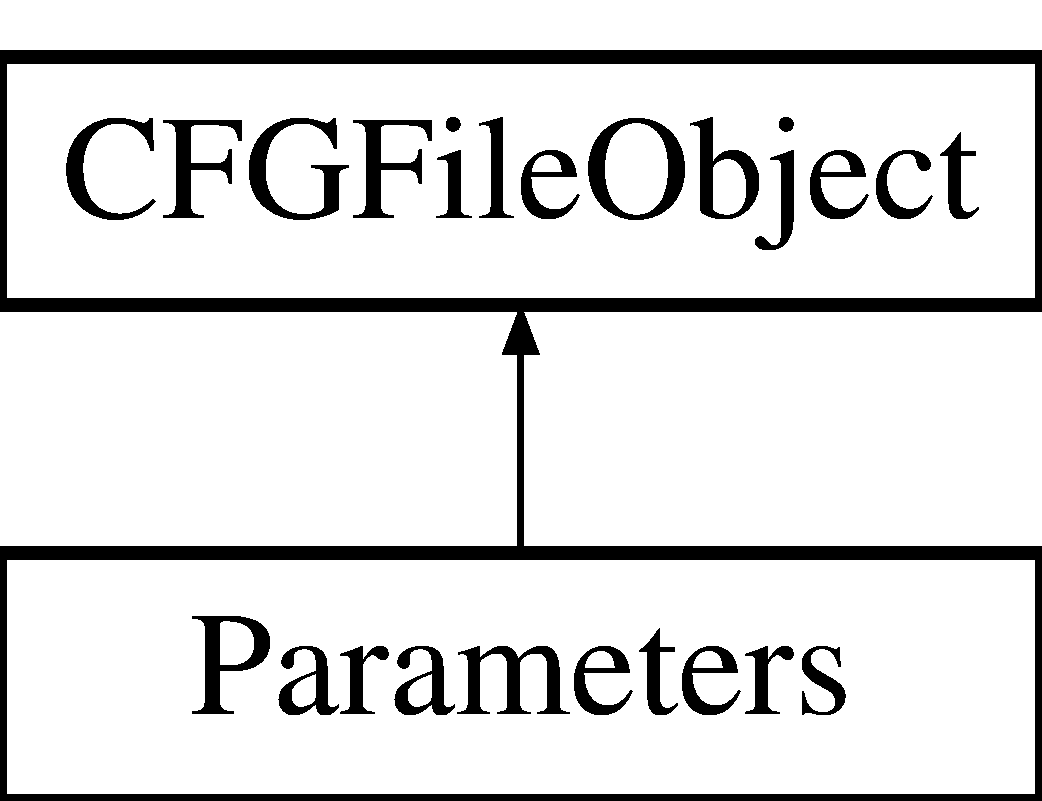
\includegraphics[height=2.000000cm]{class_c_f_g_file_object}
\end{center}
\end{figure}
\subsection*{Métodos Protegidos}
\begin{DoxyCompactItemize}
\item 
virtual std\-::ostream \& \hyperlink{class_c_f_g_file_object_aac9312bca4de84d2b2330af9857a400c}{to\-Stream} (std\-::ostream \&out)=0
\item 
virtual std\-::istream \& \hyperlink{class_c_f_g_file_object_a561dcc20e3c1db7e38868269b464ca86}{from\-Stream} (std\-::istream \&in)=0
\item 
bool \hyperlink{class_c_f_g_file_object_a4b417d2e16fc8c2c9fed64546b8b2d86}{find\-Section\-Start} (std\-::istream \&in)
\item 
bool \hyperlink{class_c_f_g_file_object_a56a717efd9097cde9bdf029b5c93e9bd}{read\-Section\-Comments} (std\-::istream \&in)
\end{DoxyCompactItemize}
\subsection*{Atributos Protegidos}
\begin{DoxyCompactItemize}
\item 
std\-::string \hyperlink{class_c_f_g_file_object_a7d62f5a9b853173c9d36e315c3de21b3}{section}
\item 
std\-::string \hyperlink{class_c_f_g_file_object_ad5bd5931f86c7843eeaca0c7a240e647}{comments}
\end{DoxyCompactItemize}
\subsection*{Amigas}
\begin{DoxyCompactItemize}
\item 
std\-::ostream \& \hyperlink{class_c_f_g_file_object_aecfe3f419c5a0b9474dfd4618323c587}{operator$<$$<$} (std\-::ostream \&out, \hyperlink{class_c_f_g_file_object}{C\-F\-G\-File\-Object} \&cfg\-File\-Object)
\item 
std\-::istream \& \hyperlink{class_c_f_g_file_object_a27640d1aa1cb5605f33a088f636af48f}{operator$>$$>$} (std\-::istream \&in, \hyperlink{class_c_f_g_file_object}{C\-F\-G\-File\-Object} \&cfg\-File\-Object)
\end{DoxyCompactItemize}


\subsection{Descrição Detalhada}
Classe base que representa uma seção de parâmetros em arquivo que armazena parâmetros. \begin{DoxyAuthor}{Autor}
Hansenclever Bassani 
\end{DoxyAuthor}


\subsection{Métodos}
\hypertarget{class_c_f_g_file_object_a4b417d2e16fc8c2c9fed64546b8b2d86}{\index{C\-F\-G\-File\-Object@{C\-F\-G\-File\-Object}!find\-Section\-Start@{find\-Section\-Start}}
\index{find\-Section\-Start@{find\-Section\-Start}!CFGFileObject@{C\-F\-G\-File\-Object}}
\subsubsection[{find\-Section\-Start}]{\setlength{\rightskip}{0pt plus 5cm}bool C\-F\-G\-File\-Object\-::find\-Section\-Start (
\begin{DoxyParamCaption}
\item[{std\-::istream \&}]{in}
\end{DoxyParamCaption}
)\hspace{0.3cm}{\ttfamily [protected]}}}\label{class_c_f_g_file_object_a4b417d2e16fc8c2c9fed64546b8b2d86}
Encontra o início de seção em uma stream. 
\begin{DoxyParams}{Parâmetros}
{\em in} & Uma stream de entrada. \\
\hline
\end{DoxyParams}
\begin{DoxyReturn}{Retorna}
Verdadeiro se encontrou o início de seção. 
\end{DoxyReturn}
\hypertarget{class_c_f_g_file_object_a561dcc20e3c1db7e38868269b464ca86}{\index{C\-F\-G\-File\-Object@{C\-F\-G\-File\-Object}!from\-Stream@{from\-Stream}}
\index{from\-Stream@{from\-Stream}!CFGFileObject@{C\-F\-G\-File\-Object}}
\subsubsection[{from\-Stream}]{\setlength{\rightskip}{0pt plus 5cm}virtual std\-::istream\& C\-F\-G\-File\-Object\-::from\-Stream (
\begin{DoxyParamCaption}
\item[{std\-::istream \&}]{in}
\end{DoxyParamCaption}
)\hspace{0.3cm}{\ttfamily [protected]}, {\ttfamily [pure virtual]}}}\label{class_c_f_g_file_object_a561dcc20e3c1db7e38868269b464ca86}
Método virtual que deve carregar esta classe de uma stream de parâmetros em texto. 
\begin{DoxyParams}{Parâmetros}
{\em in} & Uma stream de entrada. \\
\hline
\end{DoxyParams}
\begin{DoxyReturn}{Retorna}
A própria stream recebida como entrada. 
\end{DoxyReturn}


Implementado por \hyperlink{class_parameters_a1ca5a29b4ebd5a0c2a959ea28353ce07}{Parameters}.

\hypertarget{class_c_f_g_file_object_a56a717efd9097cde9bdf029b5c93e9bd}{\index{C\-F\-G\-File\-Object@{C\-F\-G\-File\-Object}!read\-Section\-Comments@{read\-Section\-Comments}}
\index{read\-Section\-Comments@{read\-Section\-Comments}!CFGFileObject@{C\-F\-G\-File\-Object}}
\subsubsection[{read\-Section\-Comments}]{\setlength{\rightskip}{0pt plus 5cm}bool C\-F\-G\-File\-Object\-::read\-Section\-Comments (
\begin{DoxyParamCaption}
\item[{std\-::istream \&}]{in}
\end{DoxyParamCaption}
)\hspace{0.3cm}{\ttfamily [protected]}}}\label{class_c_f_g_file_object_a56a717efd9097cde9bdf029b5c93e9bd}
Lê a seção de comentários 
\begin{DoxyParams}{Parâmetros}
{\em in} & Uma stream de entrada. \\
\hline
\end{DoxyParams}
\begin{DoxyReturn}{Retorna}
Verdadeiro se encontrou os comentários. 
\end{DoxyReturn}
\hypertarget{class_c_f_g_file_object_aac9312bca4de84d2b2330af9857a400c}{\index{C\-F\-G\-File\-Object@{C\-F\-G\-File\-Object}!to\-Stream@{to\-Stream}}
\index{to\-Stream@{to\-Stream}!CFGFileObject@{C\-F\-G\-File\-Object}}
\subsubsection[{to\-Stream}]{\setlength{\rightskip}{0pt plus 5cm}virtual std\-::ostream\& C\-F\-G\-File\-Object\-::to\-Stream (
\begin{DoxyParamCaption}
\item[{std\-::ostream \&}]{out}
\end{DoxyParamCaption}
)\hspace{0.3cm}{\ttfamily [protected]}, {\ttfamily [pure virtual]}}}\label{class_c_f_g_file_object_aac9312bca4de84d2b2330af9857a400c}
Método virtual que deve converter esta classe para uma stream de parâmetros em texto.


\begin{DoxyParams}{Parâmetros}
{\em out} & Uma stream de saída. \\
\hline
\end{DoxyParams}
\begin{DoxyReturn}{Retorna}
A própria stream recebida como entrada. 
\end{DoxyReturn}


Implementado por \hyperlink{class_parameters_a236265efb331f30fe0742cb1d12c22ab}{Parameters}.



\subsection{Amigas e Funções Relacionadas}
\hypertarget{class_c_f_g_file_object_aecfe3f419c5a0b9474dfd4618323c587}{\index{C\-F\-G\-File\-Object@{C\-F\-G\-File\-Object}!operator$<$$<$@{operator$<$$<$}}
\index{operator$<$$<$@{operator$<$$<$}!CFGFileObject@{C\-F\-G\-File\-Object}}
\subsubsection[{operator$<$$<$}]{\setlength{\rightskip}{0pt plus 5cm}std\-::ostream\& operator$<$$<$ (
\begin{DoxyParamCaption}
\item[{std\-::ostream \&}]{out, }
\item[{{\bf C\-F\-G\-File\-Object} \&}]{cfg\-File\-Object}
\end{DoxyParamCaption}
)\hspace{0.3cm}{\ttfamily [friend]}}}\label{class_c_f_g_file_object_aecfe3f419c5a0b9474dfd4618323c587}
Operador binário que converte um \hyperlink{class_c_f_g_file_object}{C\-F\-G\-File\-Object} em uma stream. 
\begin{DoxyParams}{Parâmetros}
{\em out} & Uma stream de saída. \\
\hline
{\em cfg\-File\-Object} & Um objeto \hyperlink{class_c_f_g_file_object}{C\-F\-G\-File\-Object}. \\
\hline
\end{DoxyParams}
\begin{DoxyReturn}{Retorna}
A própria stream recebida como entrada. 
\end{DoxyReturn}
\hypertarget{class_c_f_g_file_object_a27640d1aa1cb5605f33a088f636af48f}{\index{C\-F\-G\-File\-Object@{C\-F\-G\-File\-Object}!operator$>$$>$@{operator$>$$>$}}
\index{operator$>$$>$@{operator$>$$>$}!CFGFileObject@{C\-F\-G\-File\-Object}}
\subsubsection[{operator$>$$>$}]{\setlength{\rightskip}{0pt plus 5cm}std\-::istream\& operator$>$$>$ (
\begin{DoxyParamCaption}
\item[{std\-::istream \&}]{in, }
\item[{{\bf C\-F\-G\-File\-Object} \&}]{cfg\-File\-Object}
\end{DoxyParamCaption}
)\hspace{0.3cm}{\ttfamily [friend]}}}\label{class_c_f_g_file_object_a27640d1aa1cb5605f33a088f636af48f}
Operador binário que converte uma stream em um \hyperlink{class_c_f_g_file_object}{C\-F\-G\-File\-Object}. 
\begin{DoxyParams}{Parâmetros}
{\em in} & Uma stream de entrada. \\
\hline
{\em cfg\-File\-Object} & Um objeto \hyperlink{class_c_f_g_file_object}{C\-F\-G\-File\-Object}. \\
\hline
\end{DoxyParams}
\begin{DoxyReturn}{Retorna}
A própria stream recebida. 
\end{DoxyReturn}


\subsection{Atributos}
\hypertarget{class_c_f_g_file_object_ad5bd5931f86c7843eeaca0c7a240e647}{\index{C\-F\-G\-File\-Object@{C\-F\-G\-File\-Object}!comments@{comments}}
\index{comments@{comments}!CFGFileObject@{C\-F\-G\-File\-Object}}
\subsubsection[{comments}]{\setlength{\rightskip}{0pt plus 5cm}std\-::string C\-F\-G\-File\-Object\-::comments\hspace{0.3cm}{\ttfamily [protected]}}}\label{class_c_f_g_file_object_ad5bd5931f86c7843eeaca0c7a240e647}
Comentários de começo de arquivo. \hypertarget{class_c_f_g_file_object_a7d62f5a9b853173c9d36e315c3de21b3}{\index{C\-F\-G\-File\-Object@{C\-F\-G\-File\-Object}!section@{section}}
\index{section@{section}!CFGFileObject@{C\-F\-G\-File\-Object}}
\subsubsection[{section}]{\setlength{\rightskip}{0pt plus 5cm}std\-::string C\-F\-G\-File\-Object\-::section\hspace{0.3cm}{\ttfamily [protected]}}}\label{class_c_f_g_file_object_a7d62f5a9b853173c9d36e315c3de21b3}
Nome da sessão dos parâmetros no arquivo. 

A documentação para esta classe foi gerada a partir dos seguintes arquivos\-:\begin{DoxyCompactItemize}
\item 
Parameters.\-h\item 
Parameters.\-cpp\end{DoxyCompactItemize}

\hypertarget{class_l_h_s}{\section{Referência da Classe L\-H\-S}
\label{class_l_h_s}\index{L\-H\-S@{L\-H\-S}}
}
\subsection*{Métodos Públicos Estáticos}
\begin{DoxyCompactItemize}
\item 
\hypertarget{class_l_h_s_abdb4b724cd2d18b4a54fad05fbab245f}{static double {\bfseries next\-Double} ()}\label{class_l_h_s_abdb4b724cd2d18b4a54fad05fbab245f}

\item 
\hypertarget{class_l_h_s_a4c2b5159b4076b4f072d3c67d46eddfa}{static void {\bfseries get\-Permutation} (double min, double max, int N, Mat\-Vector$<$ double $>$ \&perm)}\label{class_l_h_s_a4c2b5159b4076b4f072d3c67d46eddfa}

\item 
\hypertarget{class_l_h_s_a0f592b00e11c6c7b202aeb92d498ccec}{static void {\bfseries get\-L\-H\-S} (const Mat\-Matrix$<$ double $>$ \&ranges, Mat\-Matrix$<$ double $>$ \&lhs, int N)}\label{class_l_h_s_a0f592b00e11c6c7b202aeb92d498ccec}

\end{DoxyCompactItemize}


A documentação para esta classe foi gerada a partir do seguinte arquivo\-:\begin{DoxyCompactItemize}
\item 
Latin\-Hypercube\-Sampling.\-h\end{DoxyCompactItemize}

\hypertarget{class_parameter}{\section{Referência da Template de Classe Parameter$<$ T $>$}
\label{class_parameter}\index{Parameter$<$ T $>$@{Parameter$<$ T $>$}}
}


{\ttfamily \#include $<$Parameters.\-h$>$}

Diagrama de Hierarquia para Parameter$<$ T $>$\-:\begin{figure}[H]
\begin{center}
\leavevmode
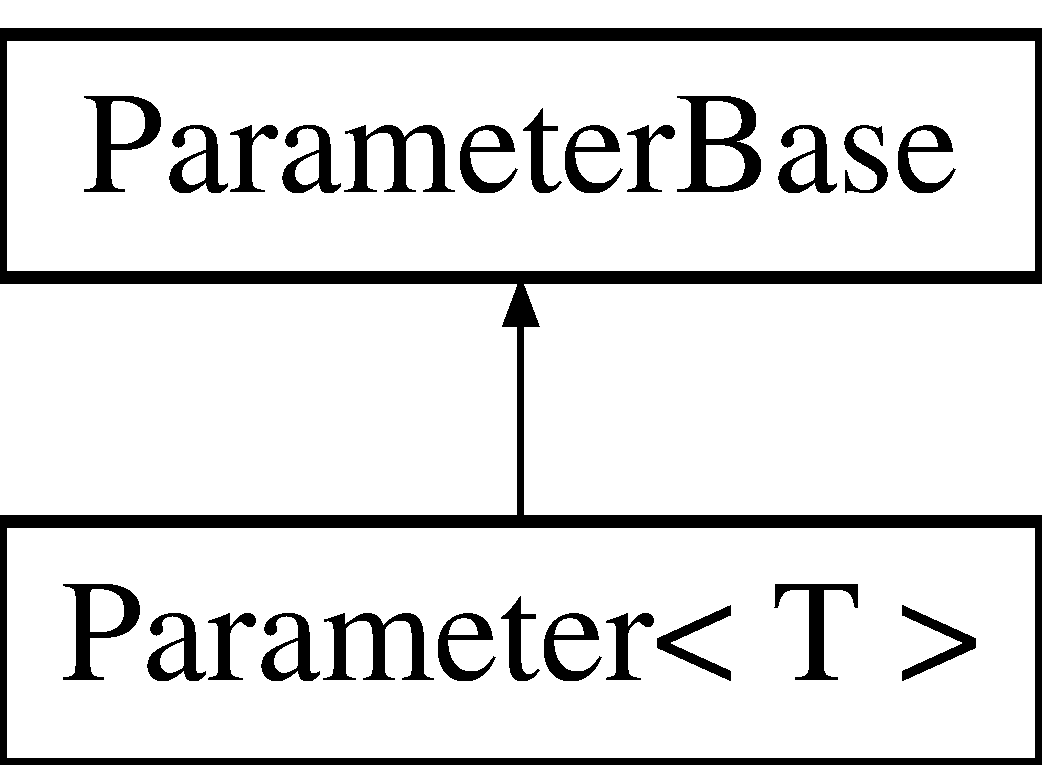
\includegraphics[height=2.000000cm]{class_parameter}
\end{center}
\end{figure}
\subsection*{Métodos Públicos}
\begin{DoxyCompactItemize}
\item 
\hypertarget{class_parameter_a39b75c306257fc9c27349e0b01a11849}{\hyperlink{class_parameter}{Parameter}$<$ T $>$ \& {\bfseries operator=} (const T \&value)}\label{class_parameter_a39b75c306257fc9c27349e0b01a11849}

\item 
\hypertarget{class_parameter_a3b15484d6beb0b7379a1c3ae987ecb59}{{\bfseries operator T} () const }\label{class_parameter_a3b15484d6beb0b7379a1c3ae987ecb59}

\item 
std\-::string \hyperlink{class_parameter_ad9328613b3f031c33ebc89e0a78356c6}{to\-String} ()
\item 
void \hyperlink{class_parameter_ab8b07f5fd7288b6803eae054f4586c32}{from\-String} (std\-::string \&str)
\end{DoxyCompactItemize}
\subsection*{Atributos Públicos}
\begin{DoxyCompactItemize}
\item 
\hypertarget{class_parameter_a5dcbb3f478f204d7931eec2b3ed66117}{T {\bfseries value}}\label{class_parameter_a5dcbb3f478f204d7931eec2b3ed66117}

\end{DoxyCompactItemize}
\subsection*{Amigas}
\begin{DoxyCompactItemize}
\item 
\hypertarget{class_parameter_a70b1cc1b148265e70223a84281bf0639}{std\-::istream \& {\bfseries operator$>$$>$} (std\-::istream \&in, \hyperlink{class_parameter}{Parameter}$<$ T $>$ \&p)}\label{class_parameter_a70b1cc1b148265e70223a84281bf0639}

\end{DoxyCompactItemize}


\subsection{Descrição Detalhada}
\subsubsection*{template$<$class T$>$class Parameter$<$ T $>$}

Classe que representa um parâmetro de tipos básicos implementando os operadores da iostream =, $<$$<$ e $>$$>$ \begin{DoxyAuthor}{Autor}
Hansenclever Bassani 
\end{DoxyAuthor}


\subsection{Métodos}
\hypertarget{class_parameter_ab8b07f5fd7288b6803eae054f4586c32}{\index{Parameter@{Parameter}!from\-String@{from\-String}}
\index{from\-String@{from\-String}!Parameter@{Parameter}}
\subsubsection[{from\-String}]{\setlength{\rightskip}{0pt plus 5cm}template$<$class T$>$ void {\bf Parameter}$<$ T $>$\-::from\-String (
\begin{DoxyParamCaption}
\item[{std\-::string \&}]{line}
\end{DoxyParamCaption}
)\hspace{0.3cm}{\ttfamily [inline]}, {\ttfamily [virtual]}}}\label{class_parameter_ab8b07f5fd7288b6803eae054f4586c32}
Método virtual nulo que lê um parâmetro a partir de uma string. 
\begin{DoxyParams}{Parâmetros}
{\em A} & string contendo um parâmetro \\
\hline
\end{DoxyParams}


Implementa \hyperlink{class_parameter_base_a949c6d70ed8893e577f492810f388073}{Parameter\-Base}.

\hypertarget{class_parameter_ad9328613b3f031c33ebc89e0a78356c6}{\index{Parameter@{Parameter}!to\-String@{to\-String}}
\index{to\-String@{to\-String}!Parameter@{Parameter}}
\subsubsection[{to\-String}]{\setlength{\rightskip}{0pt plus 5cm}template$<$class T$>$ std\-::string {\bf Parameter}$<$ T $>$\-::to\-String (
\begin{DoxyParamCaption}
{}
\end{DoxyParamCaption}
)\hspace{0.3cm}{\ttfamily [inline]}, {\ttfamily [virtual]}}}\label{class_parameter_ad9328613b3f031c33ebc89e0a78356c6}
Método virtual nulo que converte o parâmetro para uma string. \begin{DoxyReturn}{Retorna}
converte este parâmetro para uma representação de string. 
\end{DoxyReturn}


Implementa \hyperlink{class_parameter_base_a98af4bed3a47e680e51b6219b744e68b}{Parameter\-Base}.



A documentação para esta classe foi gerada a partir do seguinte arquivo\-:\begin{DoxyCompactItemize}
\item 
Parameters.\-h\end{DoxyCompactItemize}

\hypertarget{class_parameter_base}{\section{Referência da Classe Parameter\-Base}
\label{class_parameter_base}\index{Parameter\-Base@{Parameter\-Base}}
}


{\ttfamily \#include $<$Parameters.\-h$>$}

Diagrama de Hierarquia para Parameter\-Base\-:\begin{figure}[H]
\begin{center}
\leavevmode
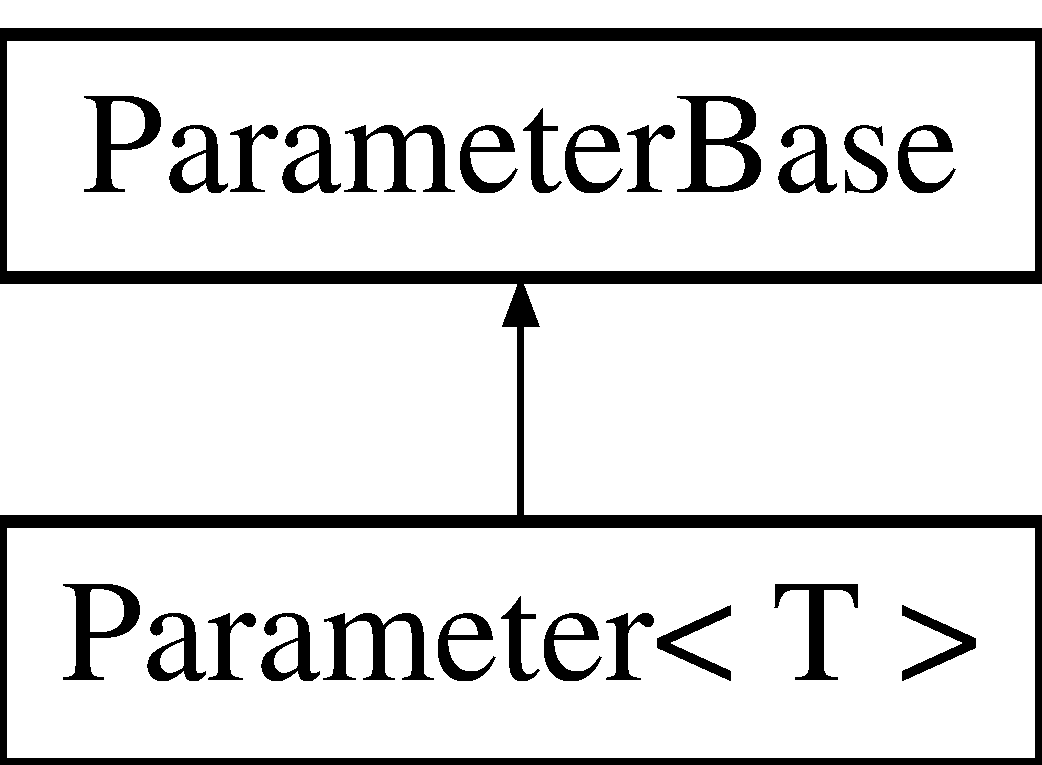
\includegraphics[height=2.000000cm]{class_parameter_base}
\end{center}
\end{figure}
\subsection*{Métodos Públicos}
\begin{DoxyCompactItemize}
\item 
virtual std\-::string \hyperlink{class_parameter_base_a98af4bed3a47e680e51b6219b744e68b}{to\-String} ()=0
\item 
virtual void \hyperlink{class_parameter_base_a949c6d70ed8893e577f492810f388073}{from\-String} (std\-::string \&line)=0
\end{DoxyCompactItemize}
\subsection*{Atributos Públicos}
\begin{DoxyCompactItemize}
\item 
std\-::string \hyperlink{class_parameter_base_a3e2e2ad34b89eabb0484b3a338133614}{name}
\item 
std\-::string \hyperlink{class_parameter_base_a6947177ee16a3821c8541635247188c5}{description}
\end{DoxyCompactItemize}


\subsection{Descrição Detalhada}
Classe base para um parâmetro \begin{DoxyAuthor}{Autor}
Hansenclever Bassani 
\end{DoxyAuthor}


\subsection{Métodos}
\hypertarget{class_parameter_base_a949c6d70ed8893e577f492810f388073}{\index{Parameter\-Base@{Parameter\-Base}!from\-String@{from\-String}}
\index{from\-String@{from\-String}!ParameterBase@{Parameter\-Base}}
\subsubsection[{from\-String}]{\setlength{\rightskip}{0pt plus 5cm}virtual void Parameter\-Base\-::from\-String (
\begin{DoxyParamCaption}
\item[{std\-::string \&}]{line}
\end{DoxyParamCaption}
)\hspace{0.3cm}{\ttfamily [pure virtual]}}}\label{class_parameter_base_a949c6d70ed8893e577f492810f388073}
Método virtual nulo que lê um parâmetro a partir de uma string. 
\begin{DoxyParams}{Parâmetros}
{\em A} & string contendo um parâmetro \\
\hline
\end{DoxyParams}


Implementado por \hyperlink{class_parameter_ab8b07f5fd7288b6803eae054f4586c32}{Parameter$<$ T $>$}.

\hypertarget{class_parameter_base_a98af4bed3a47e680e51b6219b744e68b}{\index{Parameter\-Base@{Parameter\-Base}!to\-String@{to\-String}}
\index{to\-String@{to\-String}!ParameterBase@{Parameter\-Base}}
\subsubsection[{to\-String}]{\setlength{\rightskip}{0pt plus 5cm}virtual std\-::string Parameter\-Base\-::to\-String (
\begin{DoxyParamCaption}
{}
\end{DoxyParamCaption}
)\hspace{0.3cm}{\ttfamily [pure virtual]}}}\label{class_parameter_base_a98af4bed3a47e680e51b6219b744e68b}
Método virtual nulo que converte o parâmetro para uma string. \begin{DoxyReturn}{Retorna}
converte este parâmetro para uma representação de string. 
\end{DoxyReturn}


Implementado por \hyperlink{class_parameter_ad9328613b3f031c33ebc89e0a78356c6}{Parameter$<$ T $>$}.



\subsection{Atributos}
\hypertarget{class_parameter_base_a6947177ee16a3821c8541635247188c5}{\index{Parameter\-Base@{Parameter\-Base}!description@{description}}
\index{description@{description}!ParameterBase@{Parameter\-Base}}
\subsubsection[{description}]{\setlength{\rightskip}{0pt plus 5cm}std\-::string Parameter\-Base\-::description}}\label{class_parameter_base_a6947177ee16a3821c8541635247188c5}
Valor do parâmetro. \hypertarget{class_parameter_base_a3e2e2ad34b89eabb0484b3a338133614}{\index{Parameter\-Base@{Parameter\-Base}!name@{name}}
\index{name@{name}!ParameterBase@{Parameter\-Base}}
\subsubsection[{name}]{\setlength{\rightskip}{0pt plus 5cm}std\-::string Parameter\-Base\-::name}}\label{class_parameter_base_a3e2e2ad34b89eabb0484b3a338133614}
Nome do parâmetro. 

A documentação para esta classe foi gerada a partir do seguinte arquivo\-:\begin{DoxyCompactItemize}
\item 
Parameters.\-h\end{DoxyCompactItemize}

\hypertarget{class_parameters}{\section{Referência da Classe Parameters}
\label{class_parameters}\index{Parameters@{Parameters}}
}


{\ttfamily \#include $<$Parameters.\-h$>$}

Diagrama de Hierarquia para Parameters\-:\begin{figure}[H]
\begin{center}
\leavevmode
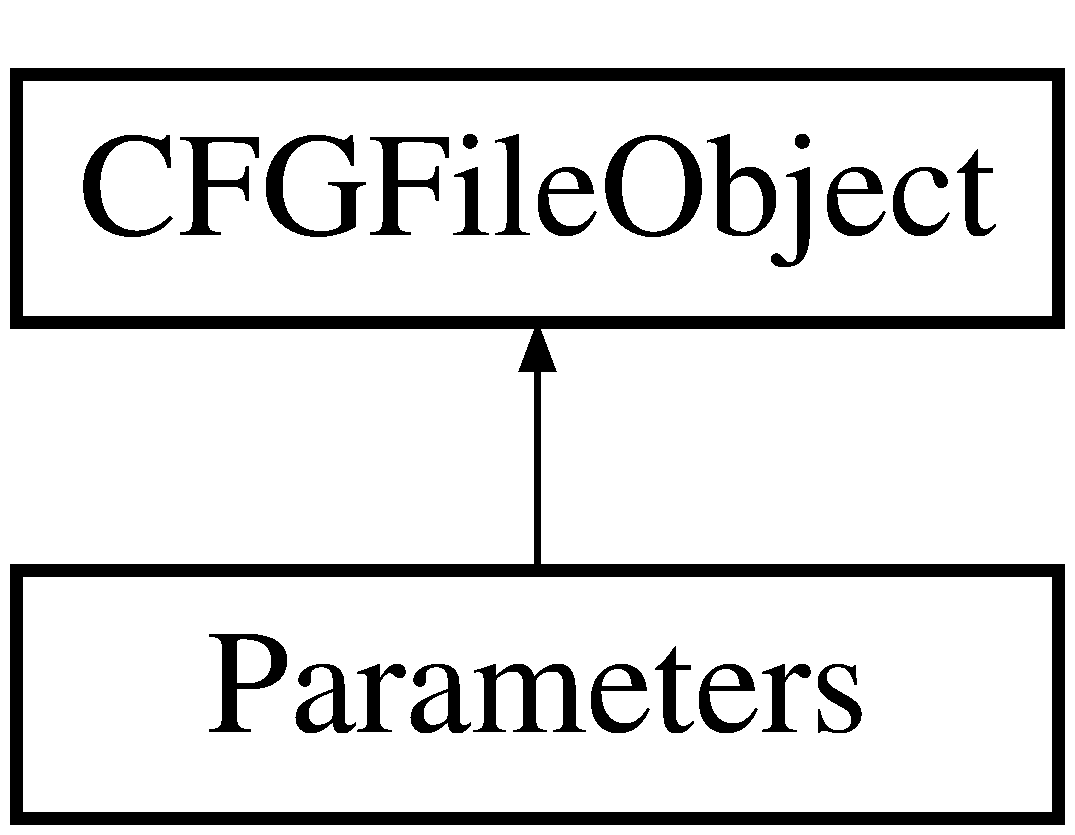
\includegraphics[height=2.000000cm]{class_parameters}
\end{center}
\end{figure}
\subsection*{Tipos Públicos}
\begin{DoxyCompactItemize}
\item 
\hypertarget{class_parameters_a2c5b67a3fff4009e404524737f52dd33}{typedef std\-::list\\*
$<$ \hyperlink{class_parameter_base}{Parameter\-Base} $\ast$ $>$ {\bfseries Parameters\-List}}\label{class_parameters_a2c5b67a3fff4009e404524737f52dd33}

\item 
\hypertarget{class_parameters_a5ef6d0faefce99751244c264f32d2821}{typedef std\-::map$<$ std\-::string, \\*
\hyperlink{class_parameter_base}{Parameter\-Base} $\ast$ $>$ {\bfseries Parameters\-Map}}\label{class_parameters_a5ef6d0faefce99751244c264f32d2821}

\end{DoxyCompactItemize}
\subsection*{Métodos Públicos}
\begin{DoxyCompactItemize}
\item 
\hyperlink{class_parameters_af4d94ee360ac0157d9065f78797fe9a1}{Parameters} ()
\item 
\hyperlink{class_parameters_aae839af2aa8d237c6b1e319ae183c982}{Parameters} (const std\-::string file\-Name)
\item 
\hyperlink{class_parameters_ac1be7d84f9e7420060cd6687c363f2dc}{Parameters} (const std\-::string file\-Name, const std\-::string \hyperlink{class_c_f_g_file_object_a7d62f5a9b853173c9d36e315c3de21b3}{section})
\item 
void \hyperlink{class_parameters_aa78d6772157b43e282a55f7e58fe0520}{add\-Parameter\-N} (\hyperlink{class_parameter_base}{Parameter\-Base} \&parameter, std\-::string name)
\item 
void \hyperlink{class_parameters_af902e19a21efb49f10287a79b624d562}{add\-Parameter\-N\-D} (\hyperlink{class_parameter_base}{Parameter\-Base} \&parameter, std\-::string name, std\-::string description)
\item 
void \hyperlink{class_parameters_a4d75e79740800b08f710657fa0e461a3}{save} (std\-::string file\-Name)
\item 
void \hyperlink{class_parameters_af77f073dabbbf334d8cb1a44f777cd73}{load} (std\-::string file\-Name)
\item 
std\-::ostream \& \hyperlink{class_parameters_a236265efb331f30fe0742cb1d12c22ab}{to\-Stream} (std\-::ostream \&out)
\item 
std\-::istream \& \hyperlink{class_parameters_a1ca5a29b4ebd5a0c2a959ea28353ce07}{from\-Stream} (std\-::istream \&in)
\end{DoxyCompactItemize}
\subsection*{Atributos Públicos}
\begin{DoxyCompactItemize}
\item 
\hypertarget{class_parameters_a9d40577daab86250d56cabfda9358e37}{Parameters\-List {\bfseries persistent\-Params}}\label{class_parameters_a9d40577daab86250d56cabfda9358e37}

\item 
\hypertarget{class_parameters_a77e1c23c11fe877234f6e31eafbd102a}{Parameters\-Map {\bfseries param\-Map}}\label{class_parameters_a77e1c23c11fe877234f6e31eafbd102a}

\end{DoxyCompactItemize}
\subsection*{Additional Inherited Members}


\subsection{Descrição Detalhada}
Classe principal de parâmetros. Esta classe representa um conjunto de parâmetros a ser armazenado em arquivo. Ela deve ser extendida e incluir parâmetros do tipo \char`\"{}\-Parameter\char`\"{} dos tipos desejados. Estes parâmetros devem ser inicializados no construtor da classe. No construtor também devem ser indicados os parâmetros que devem ser armazenados em arquivo através das funções \char`\"{}add\-Parameter\char`\"{} \begin{DoxyAuthor}{Autor}
Hansenclever Bassani 
\end{DoxyAuthor}


\subsection{Construtores \& Destrutores}
\hypertarget{class_parameters_af4d94ee360ac0157d9065f78797fe9a1}{\index{Parameters@{Parameters}!Parameters@{Parameters}}
\index{Parameters@{Parameters}!Parameters@{Parameters}}
\subsubsection[{Parameters}]{\setlength{\rightskip}{0pt plus 5cm}Parameters\-::\-Parameters (
\begin{DoxyParamCaption}
{}
\end{DoxyParamCaption}
)\hspace{0.3cm}{\ttfamily [inline]}}}\label{class_parameters_af4d94ee360ac0157d9065f78797fe9a1}
Construtor padrão \hypertarget{class_parameters_aae839af2aa8d237c6b1e319ae183c982}{\index{Parameters@{Parameters}!Parameters@{Parameters}}
\index{Parameters@{Parameters}!Parameters@{Parameters}}
\subsubsection[{Parameters}]{\setlength{\rightskip}{0pt plus 5cm}Parameters\-::\-Parameters (
\begin{DoxyParamCaption}
\item[{const std\-::string}]{file\-Name}
\end{DoxyParamCaption}
)\hspace{0.3cm}{\ttfamily [inline]}}}\label{class_parameters_aae839af2aa8d237c6b1e319ae183c982}
Construtor que carrega parâmetros de um arquivo \hypertarget{class_parameters_ac1be7d84f9e7420060cd6687c363f2dc}{\index{Parameters@{Parameters}!Parameters@{Parameters}}
\index{Parameters@{Parameters}!Parameters@{Parameters}}
\subsubsection[{Parameters}]{\setlength{\rightskip}{0pt plus 5cm}Parameters\-::\-Parameters (
\begin{DoxyParamCaption}
\item[{const std\-::string}]{file\-Name, }
\item[{const std\-::string}]{section}
\end{DoxyParamCaption}
)\hspace{0.3cm}{\ttfamily [inline]}}}\label{class_parameters_ac1be7d84f9e7420060cd6687c363f2dc}
Construtor que seta a sessão e carrega parâmetros de um arquivo 

\subsection{Métodos}
\hypertarget{class_parameters_aa78d6772157b43e282a55f7e58fe0520}{\index{Parameters@{Parameters}!add\-Parameter\-N@{add\-Parameter\-N}}
\index{add\-Parameter\-N@{add\-Parameter\-N}!Parameters@{Parameters}}
\subsubsection[{add\-Parameter\-N}]{\setlength{\rightskip}{0pt plus 5cm}void Parameters\-::add\-Parameter\-N (
\begin{DoxyParamCaption}
\item[{{\bf Parameter\-Base} \&}]{parameter, }
\item[{std\-::string}]{name}
\end{DoxyParamCaption}
)}}\label{class_parameters_aa78d6772157b43e282a55f7e58fe0520}
Adiciona à lista um parâmetro sem informar sua descrição 
\begin{DoxyParams}{Parâmetros}
{\em parameter} & Parametro \\
\hline
\end{DoxyParams}
\hypertarget{class_parameters_af902e19a21efb49f10287a79b624d562}{\index{Parameters@{Parameters}!add\-Parameter\-N\-D@{add\-Parameter\-N\-D}}
\index{add\-Parameter\-N\-D@{add\-Parameter\-N\-D}!Parameters@{Parameters}}
\subsubsection[{add\-Parameter\-N\-D}]{\setlength{\rightskip}{0pt plus 5cm}void Parameters\-::add\-Parameter\-N\-D (
\begin{DoxyParamCaption}
\item[{{\bf Parameter\-Base} \&}]{parameter, }
\item[{std\-::string}]{name, }
\item[{std\-::string}]{description}
\end{DoxyParamCaption}
)}}\label{class_parameters_af902e19a21efb49f10287a79b624d562}
Adiciona à lista um parâmetro setando seu nome e descrição 
\begin{DoxyParams}{Parâmetros}
{\em parameter} & Parametro \\
\hline
{\em name} & Nome \\
\hline
{\em description} & Descrição \\
\hline
\end{DoxyParams}
\hypertarget{class_parameters_a1ca5a29b4ebd5a0c2a959ea28353ce07}{\index{Parameters@{Parameters}!from\-Stream@{from\-Stream}}
\index{from\-Stream@{from\-Stream}!Parameters@{Parameters}}
\subsubsection[{from\-Stream}]{\setlength{\rightskip}{0pt plus 5cm}std\-::istream \& Parameters\-::from\-Stream (
\begin{DoxyParamCaption}
\item[{std\-::istream \&}]{in}
\end{DoxyParamCaption}
)\hspace{0.3cm}{\ttfamily [virtual]}}}\label{class_parameters_a1ca5a29b4ebd5a0c2a959ea28353ce07}
Método virtual que deve carregar esta classe de uma stream de parâmetros em texto. 
\begin{DoxyParams}{Parâmetros}
{\em in} & Uma stream de entrada. \\
\hline
\end{DoxyParams}
\begin{DoxyReturn}{Retorna}
A própria stream recebida como entrada. 
\end{DoxyReturn}


Implementa \hyperlink{class_c_f_g_file_object_a561dcc20e3c1db7e38868269b464ca86}{C\-F\-G\-File\-Object}.

\hypertarget{class_parameters_af77f073dabbbf334d8cb1a44f777cd73}{\index{Parameters@{Parameters}!load@{load}}
\index{load@{load}!Parameters@{Parameters}}
\subsubsection[{load}]{\setlength{\rightskip}{0pt plus 5cm}void Parameters\-::load (
\begin{DoxyParamCaption}
\item[{std\-::string}]{file\-Name}
\end{DoxyParamCaption}
)\hspace{0.3cm}{\ttfamily [inline]}}}\label{class_parameters_af77f073dabbbf334d8cb1a44f777cd73}
Lê os parâmetros de um arquivo 
\begin{DoxyParams}{Parâmetros}
{\em file\-Name} & Nome do arquivo \\
\hline
\end{DoxyParams}
\hypertarget{class_parameters_a4d75e79740800b08f710657fa0e461a3}{\index{Parameters@{Parameters}!save@{save}}
\index{save@{save}!Parameters@{Parameters}}
\subsubsection[{save}]{\setlength{\rightskip}{0pt plus 5cm}void Parameters\-::save (
\begin{DoxyParamCaption}
\item[{std\-::string}]{file\-Name}
\end{DoxyParamCaption}
)\hspace{0.3cm}{\ttfamily [inline]}}}\label{class_parameters_a4d75e79740800b08f710657fa0e461a3}
Salva os parâmetros em um arquivo 
\begin{DoxyParams}{Parâmetros}
{\em file\-Name} & Nome do arquivo \\
\hline
\end{DoxyParams}
\hypertarget{class_parameters_a236265efb331f30fe0742cb1d12c22ab}{\index{Parameters@{Parameters}!to\-Stream@{to\-Stream}}
\index{to\-Stream@{to\-Stream}!Parameters@{Parameters}}
\subsubsection[{to\-Stream}]{\setlength{\rightskip}{0pt plus 5cm}std\-::ostream \& Parameters\-::to\-Stream (
\begin{DoxyParamCaption}
\item[{std\-::ostream \&}]{out}
\end{DoxyParamCaption}
)\hspace{0.3cm}{\ttfamily [virtual]}}}\label{class_parameters_a236265efb331f30fe0742cb1d12c22ab}
Método virtual que deve converter esta classe para uma stream de parâmetros em texto.


\begin{DoxyParams}{Parâmetros}
{\em out} & Uma stream de saída. \\
\hline
\end{DoxyParams}
\begin{DoxyReturn}{Retorna}
A própria stream recebida como entrada. 
\end{DoxyReturn}


Implementa \hyperlink{class_c_f_g_file_object_aac9312bca4de84d2b2330af9857a400c}{C\-F\-G\-File\-Object}.



A documentação para esta classe foi gerada a partir dos seguintes arquivos\-:\begin{DoxyCompactItemize}
\item 
Parameters.\-h\item 
Parameters.\-cpp\end{DoxyCompactItemize}

%--- End generated contents ---

% Index
\newpage
\phantomsection
\addcontentsline{toc}{chapter}{Índice}
\printindex

\end{document}
